\documentclass[12pt]{article}
%\usepackage[document]{ragged2e}
\usepackage{array, amssymb, amsthm, linguex, enumerate, amsmath, physics, enumitem, xcolor, graphicx, xparse}
\let\fg\undefined %remove linguex/siunitx naming clash
\usepackage[english]{babel}
\usepackage[letterpaper,top=2cm,bottom=2cm,left=3cm,right=3cm,marginparwidth=1.75cm]{geometry}
\usepackage[colorlinks=true, allcolors=blue]{hyperref}
\usepackage[group-separator={,}]{siunitx} %\num{12345} -> "12,345"
\usepackage{fancyhdr}
\usepackage{notomath}
\usepackage[T1]{fontenc}
\usepackage{multicol}
\usepackage{mathtools}

%Number sets
\newcommand{\R}{\mathbb{R}}
\newcommand{\C}{\mathbb{C}}
\newcommand{\N}{\mathbb{N}}
\newcommand{\F}{\mathbb{F}}
\renewcommand{\Re}{\operatorname{Re}}
\renewcommand{\Im}{\operatorname{Im}}
\renewcommand{\L}[1]{\mathcal{L}\left({#1}\right)} %Linear Map

\newcommand{\pmp}{\,\pm\,} %add small extra space to \pm

\NewDocumentCommand{\ceil}{ s m }{% ceiling brackets
    \IfBooleanTF{#1}%
    {\lceil #2 \rceil}% starred: no-autosizing
    {\left\lceil #2 \right\rceil}% unstarred: autosizing
}

\NewDocumentCommand{\ceiling}{ s m }{% ceiling brackets
    \IfBooleanTF{#1}%
    {\lceil #2 \rceil}% starred: no-autosizing
    {\left\lceil #2 \right\rceil}% unstarred: autosizing
}

\NewDocumentCommand{\floor}{ s m }{% floor brackets
    \IfBooleanTF{#1}%
    {\lfloor #2 \rfloor}% starred: no-autosizing
    {\left\lfloor #2 \right\rfloor}% unstarred: autosizing
}

\NewDocumentCommand{\pars}{ s m }{% parenthesis
    \IfBooleanTF{#1}%
    {( #2 ) }% starred: no-autosizing
    {\left( #2 \right) }% unstarred: autosizing
}

\NewDocumentCommand{\inner}{ s m }{% inner product
    \IfBooleanTF{#1}%
    {\langle #2 \rangle}% starred: no-autosizing
    {\left\langle #2 \right\rangle}% unstarred: autosizing
}

\NewDocumentCommand{\innerconj}{ s m }{% inner product
    \IfBooleanTF{#1}%
    {\overline{\langle #2 \rangle}}% starred: no-autosizing
    {\overline{\left\langle #2 \right\rangle}}% unstarred: autosizing
}

\NewDocumentCommand{\brac}{ s m }{% brackets
    \IfBooleanTF{#1}%
    {[#2] }% starred: no-autosizing
    {\left[ #2 \right] }% unstarred: autosizing
}

%default latex bracket size naming
\newcommand{\biggbrac}[1]{\bigg[ {#1} \bigg] }
\newcommand{\bigbrac}[1]{\big[ {#1} \big] }
\newcommand{\Bigbrac}[1]{\Big[ {#1} \Big] }


\RenewDocumentCommand{\over}{ s m }{% fraction 1/arg
    \IfBooleanTF{#1}%
    {\dfrac{1}{#2}}% starred: dfrac
    {\frac{1}{#2}}% unstarred: normal frac
}

\NewDocumentCommand{\pover}{ s m }{% parenthesis around fraction (1/arg)
    \IfBooleanTF{#1}%
    {\left(\dfrac{1}{#2}\right)}% starred: dfrac
    {\left(\frac{1}{#2}\right)}% unstarred: normal frac
}

\NewDocumentCommand{\pfrac}{ s m m}{% parenthesis around fraction (arg1/arg2)
    \IfBooleanTF{#1}%
    {\left( \dfrac{{#2}}{{#3}} \right)}% starred: dfrac
    {\left( \frac{{#2}}{{#3}} \right)}% unstarred: normal frac
}


\newcommand{\Xbar}{\bar{X}}
\newcommand{\Ybar}{\bar{Y}}
\newcommand{\xbar}{\bar{x}}
\newcommand{\ybar}{\bar{y}}

\newcommand{\symint}[1]{\int_{- #1}^{#1}}

\newcommand{\limn}{\lim_{n\to\infty}}

\newcommand{\sumn}[1]{\sum_{n=#1}^{\infty}}

\newcommand{\nptl}{\frac{n \pi t}{L}}
\newcommand{\npt}{n \pi t}
\newcommand{\npto}[1]{\frac{n \pi t}{#1}}

\newcommand{\npxl}{\frac{n \pi x}{L}}
\newcommand{\bnxl}{\frac{\beta_n x}{L}}
\newcommand{\npx}{n \pi x}
\newcommand{\np}{n \pi}
\newcommand{\npxo}[1]{\frac{n \pi x}{#1}}
\newcommand{\onp}[1]{\frac{#1}{n \pi}}
\newcommand{\onps}[1]{\frac{#1}{n^2 \pi^2}}
\newcommand{\onpc}[1]{\frac{#1}{n^3 \pi^3}}
\newcommand{\npo}[1]{\frac{n \pi}{#1}}
\newcommand{\cosp}[1]{\cos \pars{#1}}
\newcommand{\sinp}[1]{\sin \pars{#1}}
\newcommand{\intll}{\int_{-L}^{L}}
\newcommand{\intl}{\int_{0}^L}

\newcommand{\gammaDist}[2]{\operatorname{Gamma} \left( {#1},{#2} \right)} %gamma distribution
\NewDocumentCommand{\normalDist}{s g g}{ %normal distibution
    \IfBooleanTF{#1} { % starred, no autosizing parenthesis
      \IfNoValueTF{#2}{
          N (\mu,\, \sigma^2 ) %\normalDist* "default" normal distribution N(\mu, \sigma^2)
        } {
            \IfNoValueTF{#3}{N (#2)}{} %\normalDist{arg} --> N(arg)
        }
      \IfNoValueTF{#3}{}{N ( #2, #3 )}  %\normalDist*{arg1}{arg2} --> N(arg1,arg2)
    }  % else (unstarred) autosize parenthesis
    {
        \IfNoValueTF{#2}{
            N \left(\mu,\, \sigma^2 \right) %\normalDist "default" normal distribution N(\mu, \sigma^2)
        } {
            \IfNoValueTF{#3}{N \left(#2\right)}{} %\normalDist{arg} --> N(arg)
        }
        \IfNoValueTF{#3}{}{N \left( #2, #3 \right)} %\normalDist{arg1}{arg2} --> N(arg1,arg2)
    }
}



%colors
\definecolor{ggreen}{RGB}{0, 127, 0}
\definecolor{dgray}{RGB}{63,63,63}
\definecolor{neonorange}{RGB}{255,47,0}
\definecolor{mygray}{rgb}{0.5,0.5,0.5}
\definecolor{eblue}{RGB}{0,74,127}
\newcommand{\red}[1]{\color{red}{#1}\color{black}}
\newcommand{\green}[1]{\color{ggreen}{#1}\color{black}}
\newcommand{\blue}[1]{\color{blue}{#1}\color{black}}
\newcommand{\setRed}{\color{red}}
\newcommand{\setBlack}{\color{black}}
\newcommand{\setBlue}{\color{blue}}
\newcommand{\setGreen}{\color{ggreen}}

\newcommand{\coshp}[1]{\cosh \pars{#1}}
\newcommand{\sinhp}[1]{\sinh \pars{#1}}
\newcommand{\cunt}{\frac{c n \pi t}{L}}
\newcommand{\absl}{\abs{\lambda}}
\newcommand{\rabsl}{\sqrt{\abs{\lambda}}}
\newcommand{\qiffq}{\quad\iff\quad}
\newcommand{\thru}[1]{{#1}_1, \dots, {#1}_n}
\newcommand{\sumThru}[1]{{#1}_1 + \cdots + {#1}_n}
\newcommand{\yn}{Y_1, \dots, Y_n} % Y_1, ..., Y_n
\newcommand{\xn}{X_1, \dots, X_n} % Y_1, ..., Y_n

%hats and tildes
\newcommand{\that}{\widehat{\theta}} % theta hat
\newcommand{\phat}{\widehat{p}} % p hat
\newcommand{\qhat}{\widehat{q}} % p hat
\newcommand{\psihat}{\widehat{\psi}} % psi hat
\newcommand{\Psihat}{\widehat{\Psi}} % Psi hat
\newcommand{\ptilde}{\widetilde{p}} % psi tilde
\newcommand{\Psitil}{\widetilde{\Psi}} % Psi tilde
\newcommand{\betah}{\widehat{\beta}} % beta hat

%2x2 matrix shortcuts
\newcommand{\detx}[4]{\begin{vmatrix}{#1} & {#2}\\{#3}&{#4}\end{vmatrix}} % 2x2 determinant
\newcommand{\dety}[9]{\begin{vmatrix}{#1} & {#2} & {#3} \\{#4}&{#5}&{#6}\\ {#7} & {#8} & {#9}\end{vmatrix}} % 3x3 determinant
\newcommand{\bmaty}[9]{\begin{bmatrix}{#1} & {#2} & {#3} \\{#4}&{#5}&{#6}\\ {#7} & {#8} & {#9}\end{bmatrix}} % 3x3 matrix
\newcommand{\bmat}[4]{\begin{bmatrix}{#1} & {#2}\\{#3}&{#4}\end{bmatrix}} % 2x2 matrix brackets
\renewcommand{\pmat}[4]{\begin{pmatrix}{#1} & {#2}\\{#3}&{#4}\end{pmatrix}} % 2x2 matrix parenthesis

%remove any enumerate/itemize indent temporarily
\makeatletter   %% <- make @ usable in macro names
\newcommand*\notab[1]{%
  \begingroup   %% <- limit scope of the following changes
    \par        %% <- start a new paragraph
    \@totalleftmargin=0pt \linewidth=\columnwidth
    %% ^^ let other commands know that the margins have been reset
    \parshape 0
    %% ^^ reset the margins
    #1\par      %% <- insert #1 and end this paragraph
  \endgroup
}
\makeatother    %% <- revert @


\newcommand{\dimrange}[1]{\operatorname{dim}\operatorname{range}{#1}} % dimrange
\newcommand{\dimnull}[1]{\operatorname{dim}\operatorname{null}{#1}} % dimnull
\newcommand{\range}[1]{\operatorname{range}{#1}} %range
\newcommand{\nullspace}{\operatorname{null}} %null

% polynomial notation
\NewDocumentCommand{\poly}{ s g g }{%
    \IfBooleanTF{#1} {
        \IfNoValueTF{#2} {
            \mathcal{P}(\mathbb{R})
        } {
            \mathcal{P}_{#2}(\mathbb{R})
        }
    } {
        \IfNoValueTF{#3} {
            {\mathcal{P}(#2)}
        } { %else
            {\mathcal{P}_{#2}(#3)}
        }
    }
}

\NewDocumentCommand{\bias}{ s m }{% bias(arg)
    \IfBooleanTF{#1}%
    {\operatorname{bias}(#2)}% starred: no autosizing
    {\operatorname{bias}\left(#2\right)}% unstarred: autosizing
}

\NewDocumentCommand{\MSE}{ s m }{% MSE(arg)
    \IfBooleanTF{#1}%
    {\operatorname{MSE}(#2)}% starred: no autosizing
    {\operatorname{MSE}\left(#2\right)}% unstarred: autosizing
}

\NewDocumentCommand{\Var}{ s m }{% variance with parenthesis V(arg)
    \IfBooleanTF{#1}%
    {\operatorname{Var}(#2)}% starred: no autosizing
    {\operatorname{Var}\left(#2\right)}% unstarred: autosizing
}

\NewDocumentCommand{\Varb}{ s m }{% variance with brackets V[arg]
    \IfBooleanTF{#1}%
    {\operatorname{Var}[\,#2\,]}% starred: no autosizing
    {\operatorname{Var}\left[\,#2\,\right]}% unstarred: has autosizing
}

\NewDocumentCommand{\Vb}{ s m }{% another renaming of variance with brackets V[arg]
    \IfBooleanTF{#1}%
    {\operatorname{Var}[\,#2\,]}% starred: no autosizing
    {\operatorname{Var}\left[\,#2\,\right]}% unstarred: has autosizing
}

\NewDocumentCommand{\E}{ s m }{% expectation with parenthesis E(arg)
    \IfBooleanTF{#1}%
    {\operatorname{E}(#2)}% starred: no autosizing
    {\operatorname{E}\left(#2\right)}% unstarred: has autosizing
}

\NewDocumentCommand{\Eb}{ s m }{% expectation with brackets E[arg]
    \IfBooleanTF{#1}%
    {\operatorname{E}[#2]}% starred: no autosizing
    {\operatorname{E}\left[#2\right]}% unstarred: has autosizing
}

\RenewDocumentCommand{\P}{ s m }{% probability with parenthesis Pr(arg)
    \IfBooleanTF{#1}%
    {\Pr (#2) }% starred: no autosizing
    {\Pr \left( #2 \right) }% unstarred: has autosizing
}

\NewDocumentCommand{\prob}{ s m }{% probability with parenthesis Pr(arg)
    \IfBooleanTF{#1}%
    {\Pr (#2) }% starred: no autosizing
    {\Pr \left( #2 \right) }% unstarred: has autosizing
}

\NewDocumentCommand{\eff}{ s m }{% efficiency with parenthesis eff(arg)
    \IfBooleanTF{#1}%
    {\operatorname{eff}(#2)}% starred: no autosizing
    {\operatorname{eff}\left(#2\right)}% unstarred: has autosizing
}

%vertical vector of up to 8 elements
\NewDocumentCommand\vvec{s m g g g g g g g}{%
    \IfBooleanTF{#1} {
        \begin{bmatrix}% if starred use brackets
            \IfNoValueTF{#2}{}{#2}
            \IfNoValueTF{#3}{}{\\#3}
            \IfNoValueTF{#4}{}{\\#4}
            \IfNoValueTF{#5}{}{\\#5}
            \IfNoValueTF{#6}{}{\\#6}
            \IfNoValueTF{#7}{}{\\#7}
            \IfNoValueTF{#8}{}{\\#8}
        \end{bmatrix}
    }  % else (unstarred) use parethesis
    {
        \begin{pmatrix}%
            \IfNoValueTF{#2}{}{#2}
            \IfNoValueTF{#3}{}{\\#3}
            \IfNoValueTF{#4}{}{\\#4}
            \IfNoValueTF{#5}{}{\\#5}
            \IfNoValueTF{#6}{}{\\#6}
            \IfNoValueTF{#7}{}{\\#7}
            \IfNoValueTF{#8}{}{\\#8}
        \end{pmatrix}
    }
}
\def\Cov{\operatorname{Cov}} %Covariance
\def\df{\text{df}} %degrees of freedom
\def\ARMA{\operatorname{ARMA}}
\def\AR{\operatorname{AR}}
\def\MA{\operatorname{MA}}
\def\ACF{\operatorname{ACF}}
\def\PACF{\operatorname{PACF}}
\def\ARiMA{\operatorname{ARiMA}}
\NewDocumentCommand{\example}{ s g }{% Example header
    \IfBooleanTF{#1}%
    {\vspace{0.1in}}% starred: 0.1in
    {\vspace{0.2in}}% unstarred: 0.2in
    \IfNoValueTF{#2} {\noindent\textbf{\color{eblue} Example: }}{\noindent\textbf{\color{eblue} Example (#2): }}
}
\NewDocumentCommand{\disc}{ s }{% Discussion header
    \IfBooleanTF{#1}%
    {\vspace{0.1in}\noindent\textbf{Discussion: } }% starred: 0.1in
    {\vspace{0.2in}\noindent\textbf{Discussion: } }% unstarred: 0.2in
}
\NewDocumentCommand{\defn}{ s }{% Definition header
    \IfBooleanTF{#1}%
    {\vspace{0.1in}\noindent\textbf{\color{neonorange} Definition: } }% starred: 0.1in
    {\vspace{0.2in}\noindent\textbf{\color{neonorange} Definition: } }% unstarred: 0.2in
}
\NewDocumentCommand{\reason}{ s }{% Reason header
    \IfBooleanTF{#1}%
    {\vspace{0.1in}\noindent\textbf{Reason:} }% starred: 0.1in
    {\vspace{0.2in}\noindent\textbf{Reason:} }% unstarred: 0.2in
}
\NewDocumentCommand{\recall}{ s }{% Recall header
    \IfBooleanTF{#1}%
    {\vspace{0.1in}\noindent\textit{Recall:} }% starred: 0.1in
    {\vspace{0.2in}\noindent\textit{Recall:} }% unstarred: 0.2in
}
\NewDocumentCommand{\remark}{ s }{% Remark header
    \IfBooleanTF{#1}%
    {\vspace{0.1in}\noindent\textit{Remark:} }% starred: 0.1in
    {\vspace{0.2in}\noindent\textit{Remark:} }% unstarred: 0.2in
}

\NewDocumentCommand{\soln}{ s }{% Remark header
    \IfBooleanTF{#1}%
    {\vspace{0.1in}\noindent\textbf{Solution: } }% starred: 0.1in
    {\vspace{0.2in}\noindent\textbf{Solution: } }% unstarred: 0.2in
}
\usepackage{cancel}
\newcommand{\proj}[2]{\operatorname{proj}_{{#1}}{#2}} %projection
\newcommand{\wideand}{\qquad \text{and} \qquad}

\newcommand{\bu}[1]{\textbf{\underline{{#1}}} } %bold underline
\newcommand{\boldit}[1]{\textbf{\textit{{#1}}} } %bold italix

% put actual quotation marks "around something"
\newcommand{\say}[1]{\textquotedblleft{#1}\textquotedblright}

% max{arg} and min{arg}
\renewcommand{\max}[1]{\operatorname{max}\left\{ #1 \right\}}
\renewcommand{\min}[1]{\operatorname{min}\left\{ #1 \right\}}

\newcommand{\Span}[1]{\operatorname{span}\left\{ #1 \right\}}

%Create a new vspace line no indent
\newcommand{\nl}{\vspace{0.1in}\noindent}
\newcommand{\nnl}{\vspace{0.2in}\noindent}
\newcommand{\nnnl}{\vspace{0.3in}\noindent}
\textwidth=7.02in
\hoffset=-.425in

\setcounter{MaxMatrixCols}{20}
\begin{document}
\pagestyle{fancy}
\fancyhf{}
\fancyhead[RO]{Matthew Wilder}
\fancyhead[LO]{MTH 427 - Homework \#8}
\fancyfoot[CO]{Page \thepage}

\noindent MTH 427 - Spring 2023
\\Assignment \#8
\\Due: Wednesday 5-3-2023


\section{Exercise text book, Shumway and Stoffer}
\textbf{Problem \#3.4}

\noindent Identify the following models as $\ARMA(p, q)$ models (watch out for parameter redundancy), and determine whether they are causal and/or invertible:
\begin{enumerate}[label=(\alph*)]
    \item $x_t = 0.8 x_{t-1} - 0.15 x_{t-2} + w_t - 0.3w_{t-1}$
   
   \soln 
    
    \noindent Rewriting the equation with the backshift operator,
    $$(1-0.8B + 0.15 B^2)x_t = (1-0.3B)w_t.$$
    Therefore, 
    $$\phi(z) = 1 - 0.8z + 0.15z^2 \qquad \text{and} \qquad \theta(z) = 1 - 0.3z.$$
    Factoring $\phi$ and equating it to $\theta$, we derive the simplified models
    $$\cancel{(1-0.3z)}(1-0.5z) = \cancel{(1-0.3z)} \quad \implies \quad \underbrace{1-0.5z}_{\phi} = \underbrace{1}_{\theta}.$$
    Therefore the simplified time series is 
    $$x_t - 0.5x_{t-1} = w_t \quad \implies \quad \ARMA(1,0).$$
    Since $\phi(z)$ has only 1 root $z=2$ and $\abs{2} > 1$, the model is causal.

    \nl Since $\theta(z)$ has no roots, the model is invertible. ($\theta(z) \neq 0 \; \forall \; z \in \C \ni \abs{z} \leq 1$.)
\vspace{0.3in}
    \item $x_t = x_{t-1} - 0.5 x_{t-2} + w_t - w_{t-1}$ 
    
    \soln 
    
    \noindent Rewriting the equation with the backshift operator,
    $$(1-B + 0.5 B^2)x_t = (1-B)w_t.$$
    Therefore $$\phi(z) = 1-z+0.5z^2  \qquad \text{and} \qquad \theta(z) = 1 -z.$$

    \nl They have no common factors, so we can conclude it is an $\ARMA(2,1)$ model.

    \nl The model is causal because $\phi(z) \neq 0 \; \forall\; z \leq 1$. In particular, the roots are 
    $$z = \frac{-(-1) \pm \sqrt{(-1)^2 - 4(0.5)(1)}}{2(0.5)} \implies z = 1 \pm i$$
    And $\abs{1 \pm i} = \sqrt 2 > 1$.

    \nl The model is not invertible because $\theta(1) = 0$ and $\abs{1} \leq 1$.
\end{enumerate}

\vspace{2in}
\noindent \textbf{Problem \#3.6}

\noindent For the $\operatorname{AR}(2)$ model given by $x_t = -0.9x_{t-2} + w_t$, find the roots of the
autoregressive polynomial, and then sketch the $\operatorname{ACF}$, $\rho(h)$.

\soln* 

\nl This can be rewritten using the backshift operator to $(1+0.9B^2)x_t = w_t$ which is
 $\operatorname{AR}(2)$ with polynomial $\phi(z) = 1+0.9z^2$ and roots $\pm \frac{\sqrt{10}}{3}$.

\nl \texttt{ACF = ARMAacf(ar=c(0, -0.9), ma=0, 50)}
\\ \texttt{plot(ACF, type="h", xlab="lag")}

\notab{\center{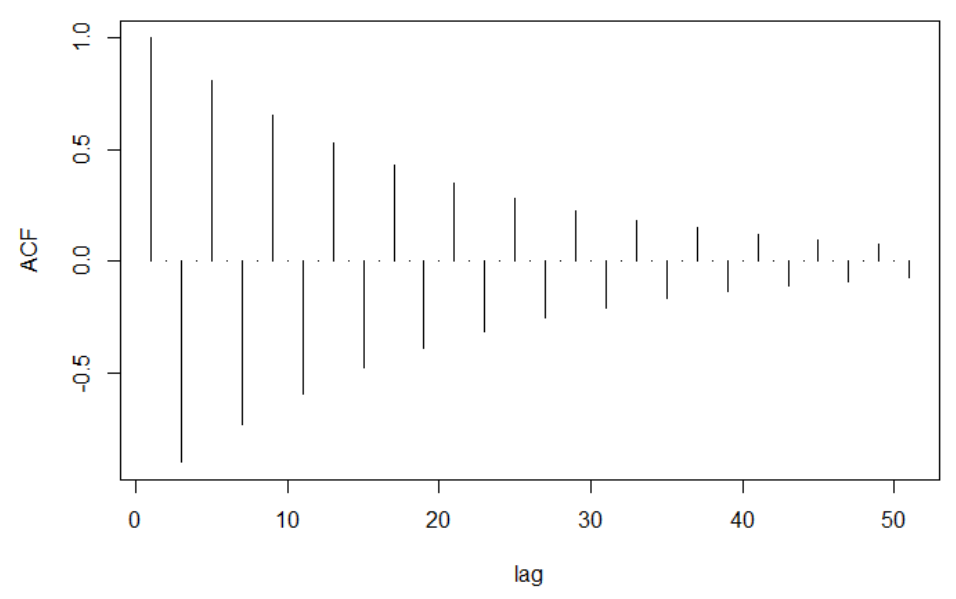
\includegraphics[width=5in]{img/acf.PNG}}}

\newpage
\noindent \textbf{Problem \#3.8}

\noindent Verify the calculations for the autocorrelation function of an $\ARMA(1, 1)$
process given in Example 3.13. Compare the form with that of the $\ACF$ for
the $\ARMA(1, 0)$ and the $\ARMA(0, 1)$ series. Plot (or sketch) the ACFs of
the three series on the same graph for $\phi = 0.6, \theta =0.9$, and comment on the
diagnostic capabilities of the $\ACF$ in this case

\noindent \soln

\nl \begin{verbatim}
par(mfrow = c(3,1))

ARMA11=arima.sim(list(order=c(1,0,1), ar=.6, ma=0.9), n=100)
acf(ARMA11)

AR1=arima.sim(list(order=c(1,0,0), ar=.6), n=100)
acf(AR1)

MA1=arima.sim(list(order=c(0,0,1), ma=0.9), n=100)
acf(MA1)
\end{verbatim}

\nl After lag 2 and lag 1 for AR and MA respectively, the series becomes mostly stationary. With the full ARMA it is only below the threshold after lag 6. Thus the MA and AR alone are better than the combination of them. Between themselves, AR is better than MA because it is easier to work with and doesnt have as many spikes outside the dashed lines.

\notab{\center{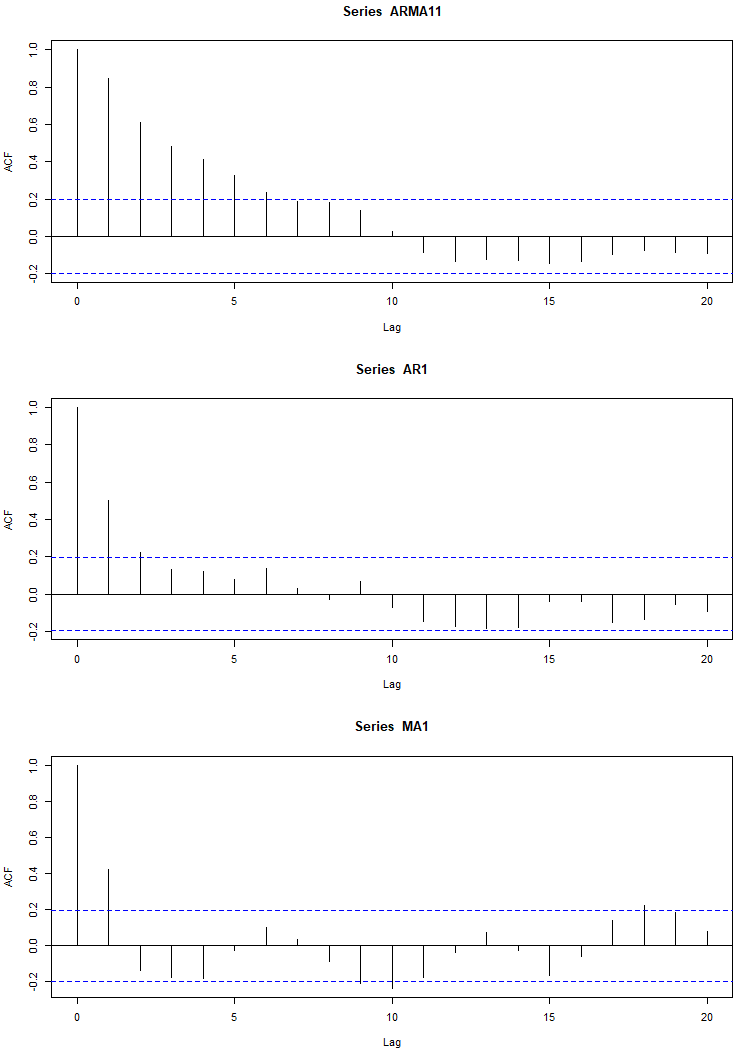
\includegraphics[width=6.75in]{img/arima.PNG}}}


\vspace{.3in}
\noindent \textbf{Problem \#3.10}

\noindent Let $x_t$ represent the cardiovascular mortality series (\texttt{cmort}) discussed in
Chapter 2, Example 2.2.

\begin{enumerate}[label=(\alph*)]
    \item Fit an AR(2) to $x_t$ using linear regression as in Example 3.17.
    
    \noindent \soln 

    \noindent \texttt{library(astsa)}
    \\ \texttt{regr = ar.ols(cmort, order=2, demean=FALSE, intercept=TRUE)}

    \nl \notab{\center{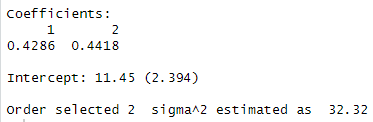
\includegraphics[width=3.5in]{img/2.PNG}}}
    \item Assuming the fitted model in (a) is the true model, find the forecasts over a four-week horizon, $x_{n+m}^n$, for $m = 1,2,3,4$, and the corresponding 95\% prediction intervals.
    
    \noindent \soln 

    \noindent \texttt{fore=predict(regr, n.ahead=4)}\\
    \texttt{ts.plot(cmort, fore\$pred, col=1:2, xlim=c(1979,1980), ylab="Cardiovascular Mortality")}\\
    \texttt{lines(fore\$pred, type="p", col=2)}\\
    \texttt{lines(fore\$pred+1.96*fore\$se, lty="dashed", col=4)}\\
    \texttt{lines(fore\$pred-1.96*fore\$se, lty="dashed", col=4)}\\

    \nl \notab{\center{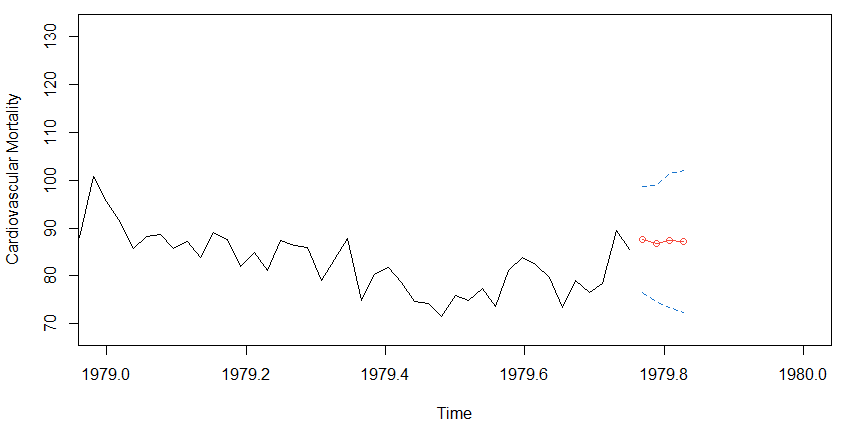
\includegraphics[width=7in]{img/4week.PNG}}}

    \nl For the exact values of the prediction intervals,
    \begin{verbatim}
        ciUpper = fore$pred+1.96*fore$se
        ciLower = fore$pred-1.96*fore$se
        
        for (m in 1:4) {
          cat("m =", m, "(", ciLower[m], ",", ciUpper[m], ")\n")
        }\end{verbatim}

        yields \begin{verbatim}
m = 1 ( 76.45756 , 98.74217 )
m = 2 ( 74.64094 , 98.88604 )
m = 3 ( 73.35405 , 101.3202 )
m = 4 ( 72.33052 , 102.0965 )
        \end{verbatim}
\end{enumerate}
\vspace{0.5in}
\section{Additional Exercises}

\subsection{Exercise (linear process representation of ARMA)}


For those models of Problem \#3.4 (text book) that are causal, compute the first four coefficients $\psi_0, \psi_1, \dots, \psi_3$ in the causal linear process representation $x_t = \sum_{j=0}^{\infty} \psi_j w_{t-j}$

\nl \soln*

\nl Since both models were causal, will complete in 2 parts.

\begin{enumerate}[label=(\alph*)]
    \item $x_t - 0.5x_{t-1} = w_t$ 
    
\begin{align*}
    & \psi_0 + \psi_1z + \psi_2z^2 + \psi_3z^3 + \cdots = \frac{\theta(z)}{\phi(z)} = \frac{1}{1-0.5z}\\
\iff \quad & (1-0.5z)(\psi_0 + \psi_1z + \psi_2z^2 + \psi_3z^3 + \cdots) = 1\\
\iff \quad &  \psi_0 + \psi_1z + \psi_2z^2 + \psi_3z^3 + \cdots - 0.5\psi_0 z -0.5 \psi_1z^2 -0.5 \psi_2z^3 -0.5 \psi_3z^4 - \cdots = 1
\end{align*}

\nl Computing the coefficients,
$$\begin{cases}
    \psi_0 = 1 & \implies \psi_0 = 1\\
    \psi_1 z - 0.5 (1) z = 0 & \implies \psi_1 = 0.5\\
    \psi_2 z^2 - 0.5(0.5)z^2 & \implies \psi_2 = 0.25\\
    \psi_3 z^3 - 0.5(0.25)z^3 & \implies \psi_3 = 0.125 
\end{cases}$$
\newpage
    \item $x_t = x_{t-1} - 0.5 x_{t-2} + w_t - w_{t-1}$ with $\phi(z) = 1 - z + 0.5z^2$ and $\theta(z) = 1 - z$.
    
    \begin{align*}
        & \psi_0 + \psi_1z + \psi_2z^2 + \psi_3z^3 + \cdots = \frac{\theta(z)}{\phi(z)} = \frac{1 - z}{1 - z + 0.5z^2}\\
    \iff \quad & (1 - z + 0.5z^2)(\psi_0 + \psi_1z + \psi_2z^2 + \psi_3z^3 + \cdots) = 1-z\\
    \iff \quad &  \psi_0 + \psi_1z + \psi_2z^2 + \psi_3z^3 + \cdots -\psi_0 z - \psi_1z^2 - \psi_2z^3 - \psi_3z^4 - \cdots\\ &\qquad + 0.5\psi_0z^2 + 0.5\psi_1z^3 + 0.5\psi_2z^4 + 0.5\psi_3z^5= 1 - z
    \end{align*}
    
    \nl Computing the coefficients,
    $$\begin{cases}
        \psi_0 = 1 & \implies \psi_0 = 1\\
        \psi_1 z - (1) z = -z & \implies \psi_1 = 0\\
        \psi_2 z^2 - (0)z^2 + 0.5(1)z^2 = 0 & \implies \psi_2 = -0.5\\
        \psi_3 z^3 - (-0.5)z^3 + 0.5(0)z^3 = 0& \implies \psi_3 = -0.5 
    \end{cases}$$
\end{enumerate}

\end{document}
